
%%%%%%%%%%%%%%%%%%%%%%%%%%%%%%%%%%%%%%%%%%%
                     %%% FUNCTIONS %%%
\chapter {Functions}
Sets are collections. Functions take you from one set to another.



\begin {definition} [Function] \index{function} \index{mapping} \index{transformation}
Let $A$ and $B$ be non-empty sets. A \textit{function} $f$ from $A$ to $B$ is an assignment of exactly one element in $B$ to each element in $A$. The set $A$ is called the domain of the function and the set $B$ is called the co-domain. The element from the domain, $a$ is called the pre-image and the element $b$ from the co-domain is called the target or image. The set of all images is called the range (note difference from co-domain). Functions are sometimes called \textbf{mappings} or \textbf{transformations}. The notation $a \mapsto b$ is used to denote the association of a pre-image $a$ to an image $b$.
\end {definition} 

\begin {definition}[Domain, codomain, preimage, image, range] \index{domain}\index{codomain}\index{preimage}\index{image}\index{range}
If $f$ is a function from $A$ to $B$, we say that $A$ is the \textit{domain} of $f$ and $B$ is the \textit{codomain} of $f$. If $f(a)=b$, we say that $b$ is the \textit{image} of $a$ and $a$ is the \textit{preimage} of $b$. The \textit{range},or \textit{image}, of $f$ is the set of all images of elements of $A$. Also, if $f$ is a function from $A$ to $B$,we say that $f$ \textit{maps} $A$ to $B$.

 We denote the image of $S$ by $f(S)$, so
 $$f(S)=\{t \mid \exists x \in S (t=f(s))\}$$
 We also use the shorthand $\{f(s) \mid s \in S\}$ to denote this set. 
\end {definition}

\begin {definition}[function equality]\index{function equality}
Two functions are \textbf{equal} when they have the same domain, have the same codomain, and map each element of their common domain to the same element in their common codomain.
\end {definition}
Note that if we change either the domain or codomain they are different functions.

Note that $f_1 + f_2)$ and $f_1 f_2$ are defined for real and integer valued functions.

\subsection {Set Builder Notation for Functions}



\subsection {Function signature, Function definition}
The signature of the function gives the function name, the domain and the co-domain and is written as:
$$f:A \rightarrow B$$ 
where $f$ is the function name, $A$ is the domain and $B$ is the co-domain and is read ``the function f from A to B''. \\
assigned\_grade: \{students\} $\rightarrow$ \{grades\}\\
The function definition gives the information needed to determine which element from the co-domain is the image of the element from the domain. This is called the function definition. 
$$f(a)=b$$

In pseudocode function signature is represented in the header for a function
$$floor (someValue:real): integer $$
The function definition is usually given in the block which follows but sometimes the signature can be used by itself as is done with C. Note that the type definitions are equivalent to the domain and codomains of the function.

\subsection {Function Equality}\index{function equality}

\subsection {Functions are subsets of set cross products, maplets}
All functions are subsets of the cross product of the domain and co-domain. A listing of all pairs is a valid function definition as is a table. Some authors will note specific mappings from an element a in the domain to the element b in the co-domain with the maplet notation:
$$ a \mapsto b$$ 



Sometimes we want to 

domain, co-domain, image, target, maplet, scope
function signature versus definition
graphic representation, arrow diagrams
well defined/proper function, partial functions
functional equality
graphic representation, analytic geometry (recognizing incomplete functions and non-functions)
Function versus operator

$f:S \rightarrow T$
The function f is a function that takes an argument from the set S and gives a result from the set T. S is the domain and T is the co-domain.

For function application we typically write $f(s)=t$ where $t$ is some expression based on $s$ and a method by which we can determine the unique element $t$ that $s$ maps to and can define the function using this notation. For example the function f might double the argument and add one which can be expressed as:

$f(x) = 2*x + 1$

When x is bound to a value, it results in a maplet from a member of the domain to some member in the codomain.

$f(2)=5$
or maplet $2 \mapsto 5$

For finite functions note that a function can be fully defined just by listing all the maplets of the function.

 

\


\section {Properties of Functions}
    \begin{definition}[Onto or Surjective]\index{onto} \index{surjective}
    A function $f$ from $A$ to $B$ is called \textit{onto}, or a \textit{surjection}, if and only if for every element $b \in B$ there is an element $a \in A$ with $f(a)=b$. A function $f$ is called \textit{surjective} if it is onto.
    \end{definition}

    \begin{notes}
    A function $f$ is onto if $\forall y \exists x(f(x)=y)$, where the domain for $x$ is the domain of the function and the doman for $y$ is the codomain of the function.
    \end{notes}

\begin{definition}[One-to-One, Into, Injective] \index{one-to-one} \index{into} \index{injective}
A function $f$ from $A$ to $B$ is said to be \textit{one-to-one}, \textit{into}, or \textit{injective}, if and only if $f(a)=f(a)$ implies that $a=b$ for all $a$ and $b$ in the domain of $f$. A function is said to be an \textit{injection} if it is one-to-one.
\end{definition}

\begin{definition}[One-to-One-Correspondence, One-to-One-Mapping, Bijective] \index{one-to-one correspondence}\index{bijective}
A function $f$ from $A$ to $B$ is said to be \textit{one-to-one correspondence}, or \textit{bijection}, if it is both one-to-one and onto. 
\end{definition}

\begin{figure}[htbp]
   \centering
   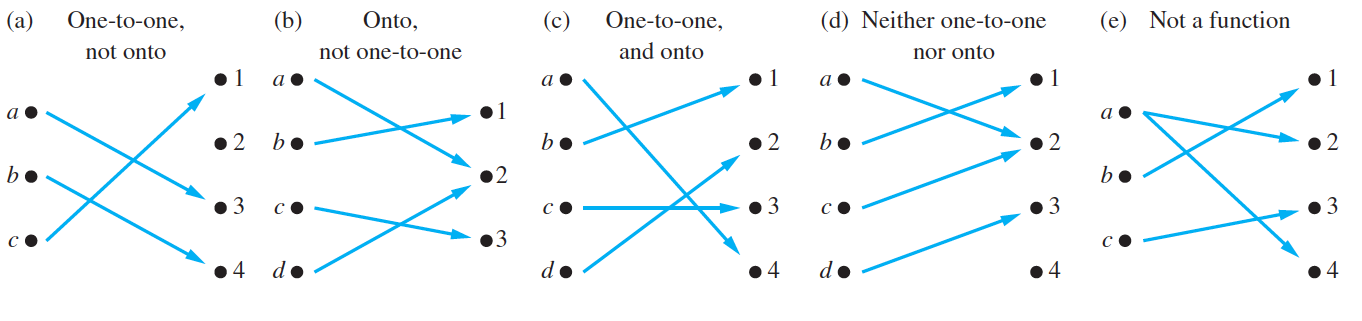
\includegraphics [width=6.5in]{Figure-2-3-5-TypesOfCorrespondences}
   \caption{Types Of Correspondences}
   \label{figure:Figure-2-3-5-TypesOfCorrespondences}
\end{figure}

    \subsection {Inverse of a Function}
    \begin{definition}[Inverse of a Function] \index{inverse of a function}
    Let $f$ be a One-to-One-Correspondence from the set $A$ to the set $B$. The inverse function of
$f$ is the function that assigns to an element $b$ belonging to $B$ the unique element $a$ in $A$
such that $f (a) = b$. The inverse function of $f$ is denoted by $f^{-1}$. Hence, $f^{-1} (b) = a$ when
$f (a) = b$.
    \end{definition}

\begin{definition}[Increasing and Strictly Increasing Functions]
A function $f$ whose domain and codomain are subsets of the set of real numbers is called \textit{increasing} if $f(x) \le f(y)$, and \textit{strictly increasing} if $f(x) < f(y)$, whenever $x<y$ and $x$ and $y$ are in the domain of $f$. (The word \textit{strictly} in this definition indicates a strict inequality.)
\end{definition}

\section {Composition of Functions}
\begin{definition} [Composition of Functions] \index{function composition}
Let $g$ be a function from the set $A$ to the set $B$ and let $f$ be a function from the set $B$ to the set $C$. The \textit{composition} of the functions $f$ and $g$, denoted by $f \circ g$, id defined by 
$$(f\circ g)(a)=f(g(a)).$$
\begin{notes}
Note that function composition is right-associative and that $f\circ g \ne g \circ f$. Note that the composition operator is a function which takes other functions as operands and returns a function. This is called treating functions as first-class objects in object oriented languags. Not all programming languages offer this ability.
\end{notes}
\end{definition}




\section {Common functions in computer science}

We are used to the functional notation of algebra
$$  g(x,y)$$
We are also accustomed to operators from programming languages
$$x+y$$
If the function g is defined as the sum of the two arguments, the two notations mean the same thing. The second form is called operation notation and works well for both binary and unary operators. But for arguments of more than 2 it is difficult to use. Note that the usual form is infix. But if we adopt a different convention, putting the operator after all the arguments, it is now possible to have functions of any number of arguments written in operator notation with no loss of precision. If the operator follows the operands, the notation is called post-fix. If the operator preceeds the operands, it is called prefix. Thus the function notation, prefix, infix, and suffix notation for addition are
$$+(a,b)$$
$$ab+$$
$$a+b$$
$$+ab$$
Note that the C language has a way of converting a symbol into an infix operator for a binary function.

We make special note of the important distinctions between common programming languages and the mathematical functions they implement. First, it is obvious that the mathematical convention of juxtaposing operands as implied multiplication does not work for computer languages which are not constrained to single character variables. Therefore the usual convention of an explicit multiplication operation, most always *, is adopted. Next is the challenge of differentiating between regular division and integer division. Several operators are employed in various languages and texts and sometimes is only implied by the type of the returned value. In many languages the type of the value to be returned value is infered by the types of the operands. Therefore an integer divided by an integer returns an integer, a case of integer division. To overcome this we see the apparently odd truth that $4/3 \ne 4.0/3$ in many languages. A more rigorous approach is delayed until the chapter on number theory but we define integer division in this chapter to connect the material more closely to contemporary coding practice.

	\subsection{Functions between Natural Numbers or Integers}
	\begin{displaymath}
	\text{Factorial}(n) = \prod_{i=1}^n i
	\end{displaymath}
	The remainder function is that function which returns the remainder when doing integer division. We will formally define this in the unit on Integers.
	
    \subsection {Functions of Real to Integer}
    
    \begin{definition} [Floor and Ceiling Functions]
    The \textit{floor function} assigns to the real number $x$ the largest integer that is less than or equal to $x$. The value of the floor function at $x$ is denoted by $\lfloor x \rfloor$. The \textit{ceiling function} assigns to the ral number $x$ the smallest integre that is greater than or equal to $x$. The value of the celing function at $x$ is denoted by $\lceil x \rceil$.
    
    The floor function is sometimes called the \textit{greates integer function}. It may be denoted by $[x]$. 
    \end{definition}
    
    
   \begin{table}[htbp]
   \centering
   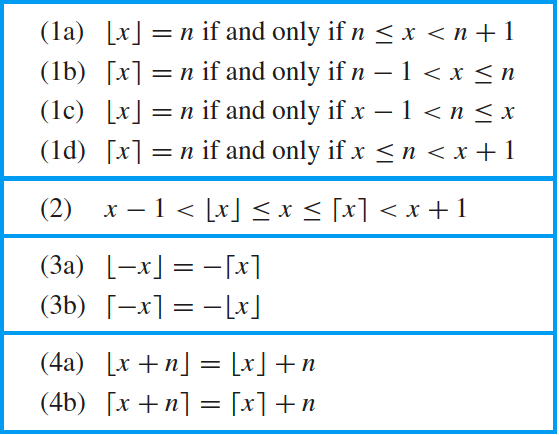
\includegraphics [width=3in]{Table-2-3-1-PropertiesOfFloorAndCeilingFunctions}
   \caption{Useful Properties of the Floor and Ceiling Functions}
   \label{table:UsefulPropertiesOfTheFloorAndCeilingFunctions}
   \end{table}

    

    \subsection{Functions between Boolean and Integer}
    ASCII is a 7-bit character set containing 128 characters. It contains the numbers from 0-9, the upper and lower case English letters from A to Z, and some special characters. The character sets used in modern computers, in HTML, and on the Internet, are all based on ASCII.
    
Boolean $\leftrightarrow$ Integer
\begin{table}[htbp]
   \centering
   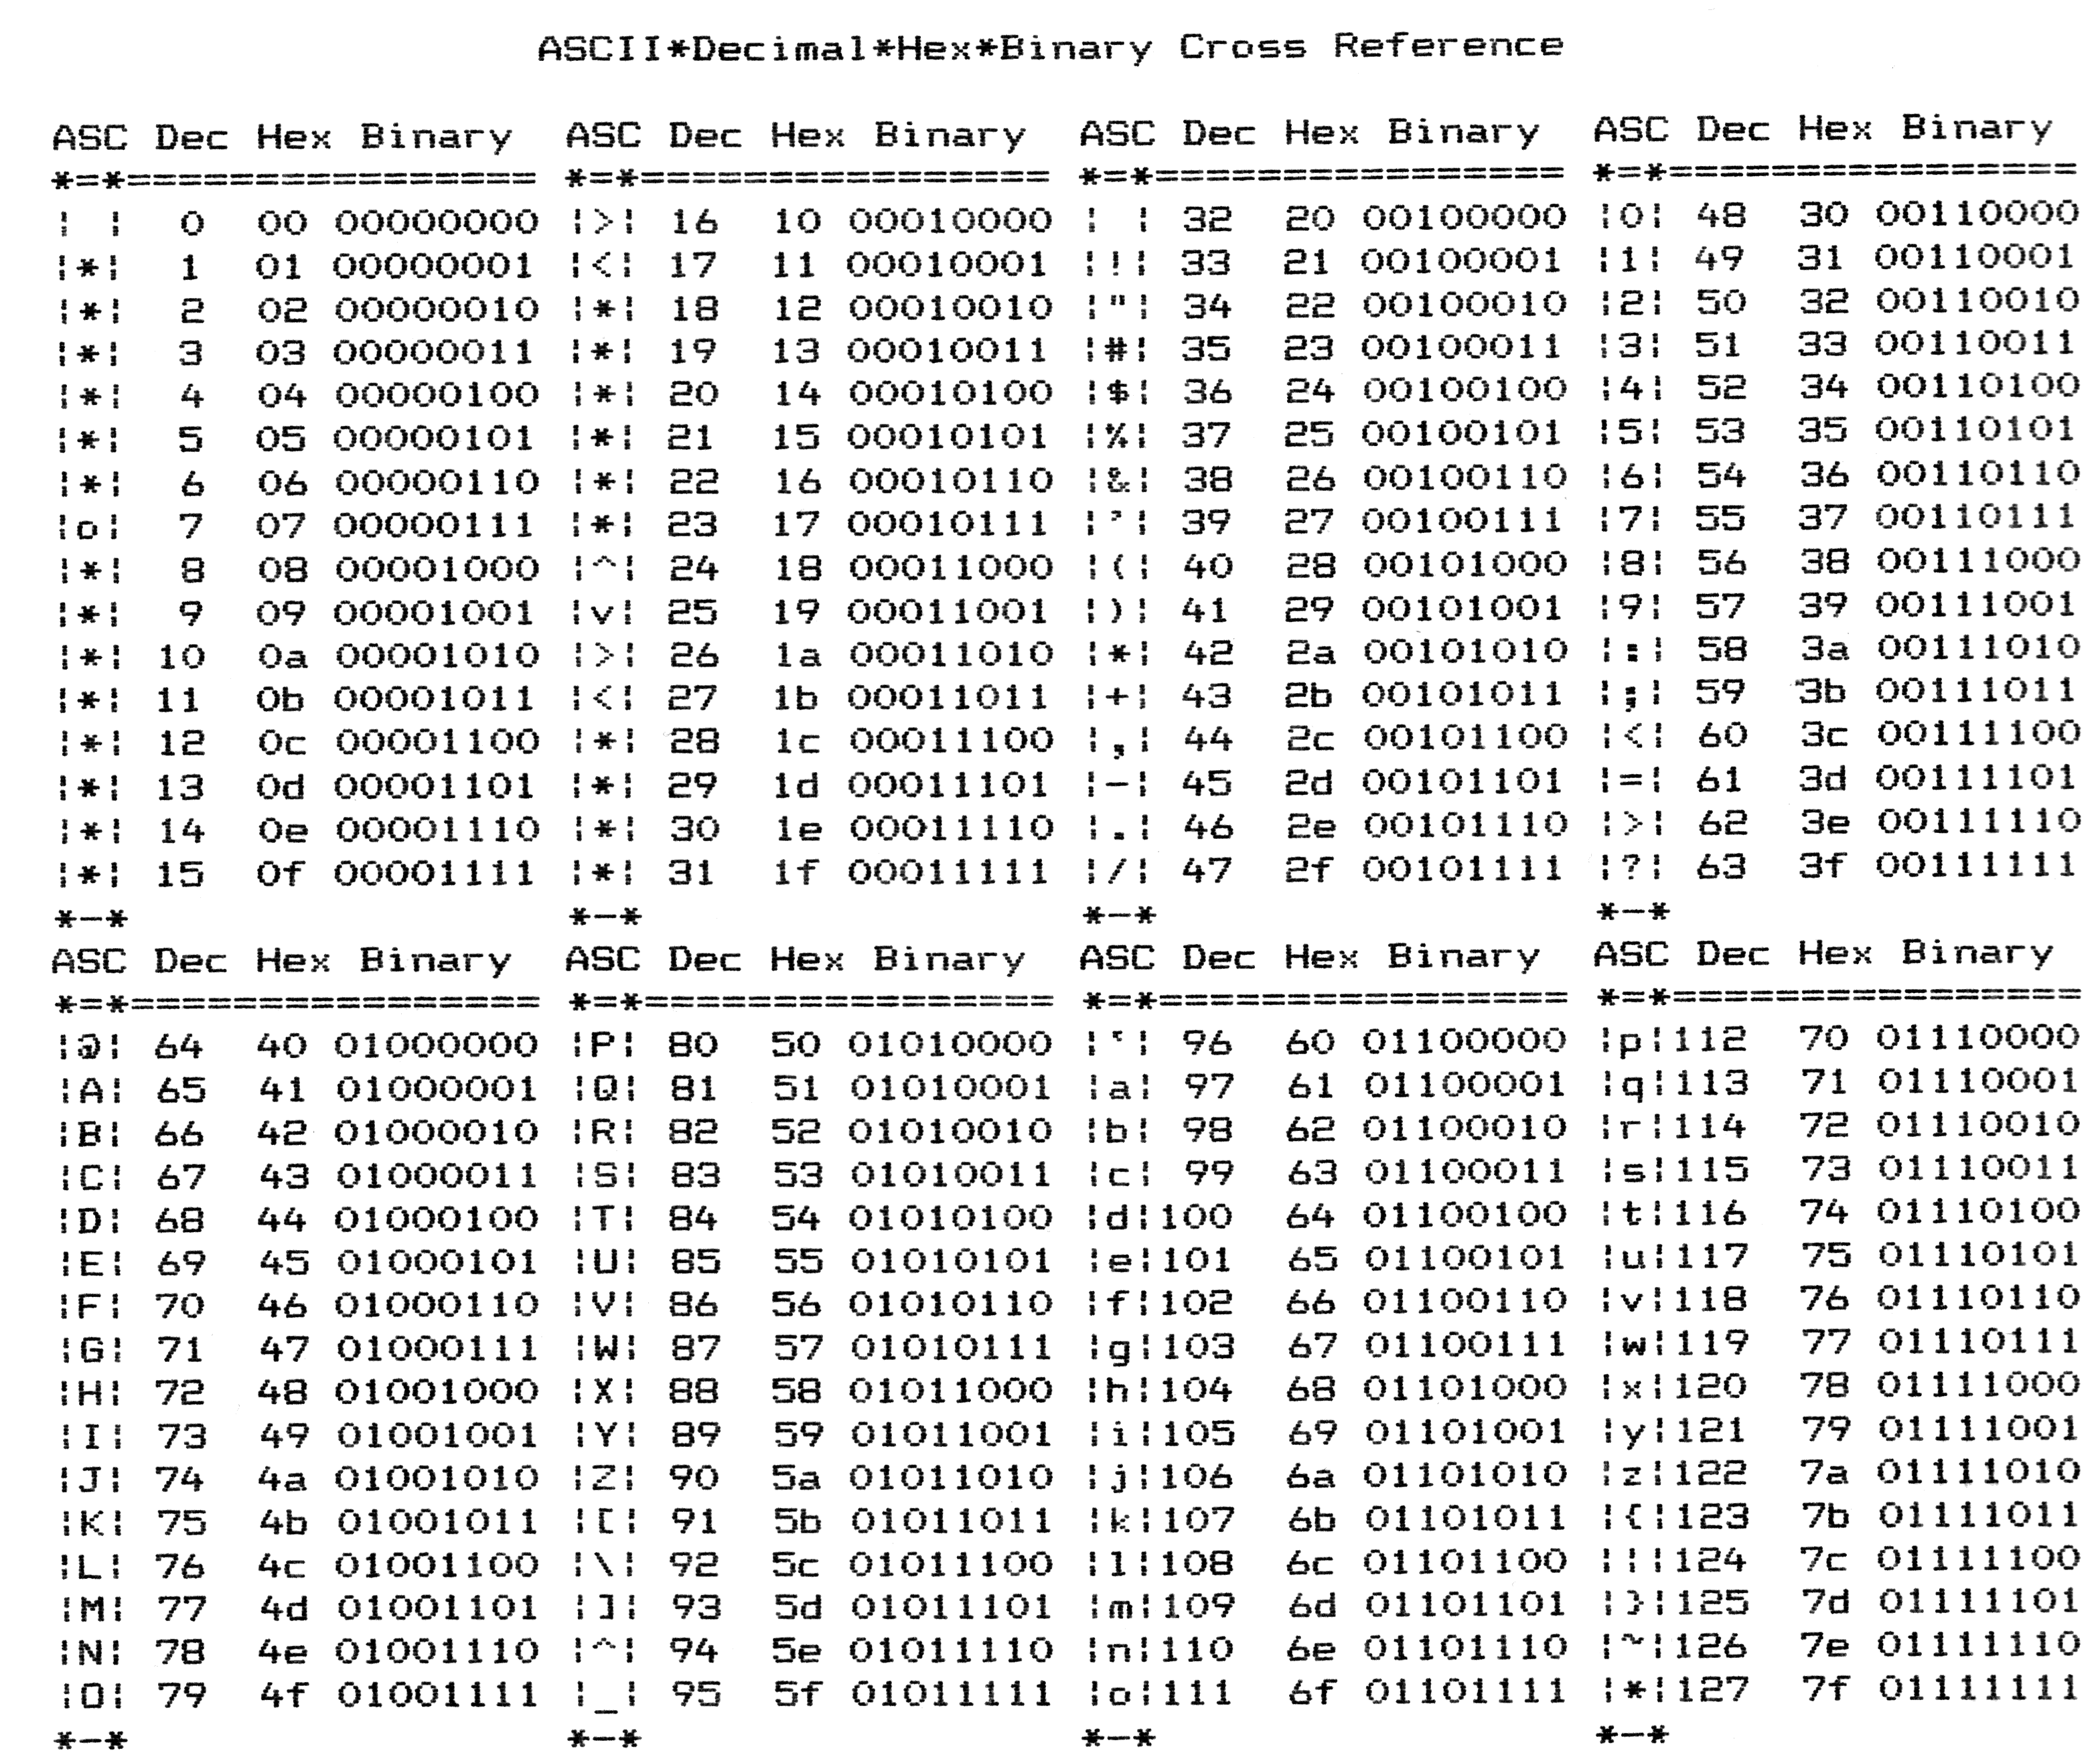
\includegraphics [width=5in]{asciifull}
   \caption{ASCII: American Standard Code for Information Interchange, 7-bit}
   \label{table:ASCIITable}
   \end{table}

    \subsection {Functions Between Boolean and Real}
Boolean $\leftrightarrow \mathbb{R}$ 

    \subsection {Functions of Real to Real}
polynomial, log, log-linear, exponential
increasing/decreasing versus strictly increasing and decreasing
cipher function
permutation function

	\subsection{Other Useful Functions}
	\begin{definition}[Characteristic Function]
	Let $S$ be a subset of a universal set $U$. The \textbf{characteristic function} $f_S$ of $S$ is the function from $U$ to the set $\mathbb{B}$ such that $f_S(x) =0$ if $x$ does not belong to $S$ and $f_S(x)=1$ when $x$ does belong to $S$.
	\end{definition}



\section {Composition of Functions}

Properties of Functions: Onto, One-to-One, One-to-One Correspondence, Invertible
An invertible function is called a permutation

Elementary Functions Used in Computer Science and Engineering
exponential and logarithmic, floor and ceiling, integer and absolute value, remainder function (MOD operator in programming), integer to binary and binary to integer, from natural numbers to integers.

It helps to note that when specifying function composition we begin to speak of the function like an operand. For example we can define a function $h$ as the composition of two other functions $f$ and $g$ using the composition operator. In functional notation we call this treating a function as a first class object, that is, the function is an object no different than other operands but simply drawn from the set of functions.

\begin{figure}[htbp]
   \centering
   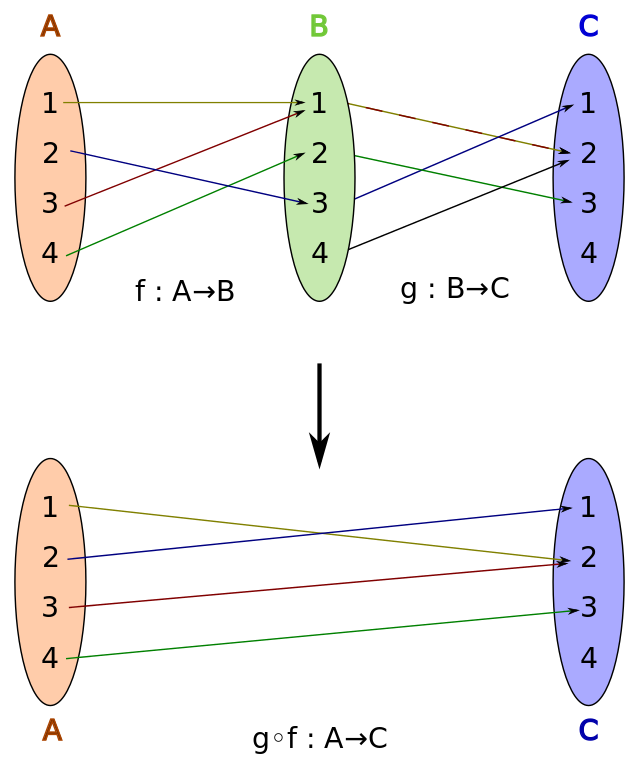
\includegraphics [width=3in]{Example_for_a_composition_of_two_functions}
   \caption{Function Composition}
   \label{figure:ExampleForACompositionOfTwoFunctions}
\end{figure}


subsection {Total and Partial Functions}
A total function is one that has a maplet for every element in the domain. These are called well defined functions. Some functions are undefined for some elements in the domain and these are called partial functions. Note that division on two numbers is a partial function. It is represented by an line through the arrow from domain to co-domain.

Not every element in the co-domain may be the image of an element in the domain. The set of all images is called the scope of the function.

\begin{definition}[Partial Function]\index{partial function}
A \textit{partial function} $f$ from a set $A$ to a set $B$ is an assignment to each element $a$ in a subset of $A$, called the \textit{domain of definition} of $f$ , of a unique element $b$ in $B$. The sets $A$ and $B$ are called the \textit{domain} and \textit{codomain} of $f$ , respectively. We say that $f$ is \textit{undefined} for elements in $A$ that are not in the domain of definition of $f$. When the domain of definition of $f$ equals $A$, we say that $f$ is a \textit{total function}. The notation $h:A \nrightarrow B$ is often used as a notation to designate a partial function $h$ that maps the set $A$ to $B$ where the set $A$ has undefined elements for the function $h$. However some authors use the same notation for partial functions as they do for partial functions.
\end{definition}



\section {Visual Representations of Functions: Set~mappings~and~analytic~geometry}
    In analytic geometry we speak of the graph of a function when we talk about ploting it against two or more axes. Note that in discrete math we will use the term \textit{graph} in a different way which does not mean the same thing.  
    
   \begin{figure}[htbp]
   \centering
   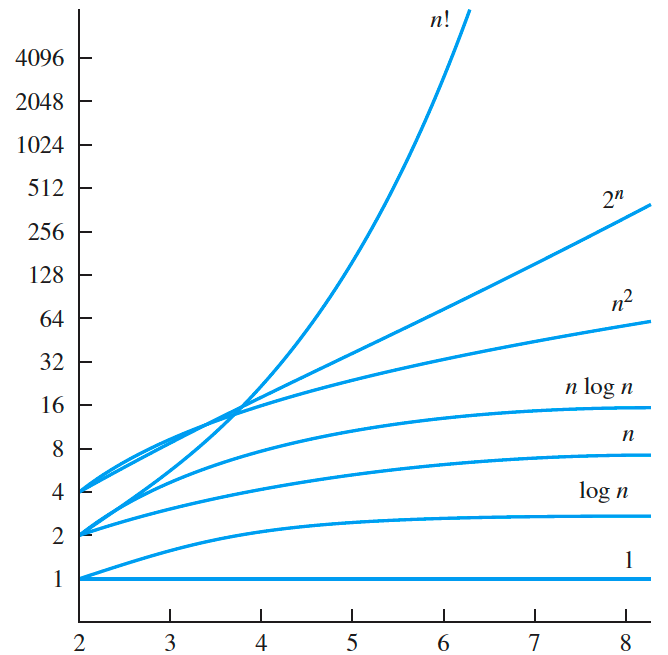
\includegraphics [width=4in]{Figure-3-2-3-GrowthOfFunctions}
   \caption{Graphs of Common Functions Needed In Computer Science}
   \label{figure:GraphsOfCommonFunctions}
\end{figure}

\section {Sequences}
Formally, a sequence can be defined as a function whose domain is either the set of the natural numbers (for infinite sequences) or the set of the first n natural numbers (for a sequence of finite length n). The position of an element in a sequence is its rank or index; it is the natural number from which the element is the image. It depends on the context or a specific convention, if the first element has index 0 or 1. When a symbol has been chosen for denoting a sequence, the nth element of the sequence is denoted by this symbol with n as subscript; for example, the nth element of the Fibonacci sequence is generally denoted $F_n$.

Like tuples, these are ordered lists. Unlike tuples, they vary in length and notation.

\begin{definition} [Sequence] \index{sequence}\index{term}
A \textit{sequence} is a function from a subset of the integers to a set $S$. We use the notation $a_n$ to denote the image of the integer $n$. We call $a_n$ a \textit{term} of the sequence. 

We use the notation $\{a_n\}$ to describe the sequence. Note how this conflicts with set notation. Note how there is no requirement that the set $S$ be numeric. We often describe sequences by listing the terms of the sequence in order of increasing subscripts.
\end{definition}

\begin{definition}[Geometric Progression]\index{geometric progression}\index{initial term}\index{common ratio}
A \textit{geometric progression} is a sequence of the form
$$ar^0,ar^1,ar^2, \dots ,ar^n, \dots$$
where the \textit{initial term} $a$ and the \text{common ratio} $r$ are real numbers.
\end{definition}

Sequences of the form $a_1, a_2, . . . , a_n$ where the terms are drawn from some set of symbols rather than numbers are often used in computer science. These finite
sequences are also called \textit{strings}. This string is also denoted by $a_1a_2 . . . a_n$. (Recall that bit strings, which are finite sequences of bits, were introduced in Section 1.1.) The length of a
string is the number of terms in this string. The empty string, denoted by $\lambda$, is the string that has no terms. The empty string has length zero.

\subsection{Special Integer Sequences}
A common technique needed in programming is finding an algorithm that will generate a particular sequence. This is the same as finding a function to do the same substituting the index variable for the loop counter. 

Trying to guess the function that can be used to create the sequence is a common test item. Note that an infinite number of sequences can be created that begin with the same few terms that are given. Still it is important to be able to quickly recognize the most common sequences and functions such as arithmetic and geometric progressions. 




In mathematics a \textit{finite sequence} is usually defined as any function $f$ whose domain is a finite initial set $\{1,2,3, \dots ,n\}$ of positive integers. The number $n$ of integers in the domain of $f$ is the \textit{length} of $f$. When considering $f$ as a finite sequence it is customery to write
$$f_1,f_2, \dots$$
rather than
$$f(1),f(2), \dots$$
in designating the value of $f$ at 1,2, \dots.

Along with this subscript notation there is the \textit{n-tuple} notation
$$(f_1,f_2, \dots f_n)$$


$f_i$ is the $i_{th}$ \textit{entry} or \textit{term} of $f$. This \textit{n-tuple} notation indicates how explicit short finite sequences can be defined and pictured. For example, the equation  
$$x=(5,1,4,0)$$
tells us that $x$ is the finite sequence of length 4 whose values on its domain \{1,2,3,4\} are given by
$$x_1=x(1)=5$$
$$x_2=x(2)=1$$
$$x_3=x(3)=4$$
$$x_4=x(4)=0$$

The most common domain for a sequence is $\mathbb{N}$. However it is frequently more convenient to use natural numbers including zero. There is an edge case where sometimes the domain is the null set in which case the sequence is empty and can be shown using a pair of empty parentheses to emphasize that there are no terms in the sequence
$$(  )$$

Consider a function $\sigma:\mathbb{N} \rightarrow \mathbb{Z}$
For example sigma(x)=2*x
this gives maplets 1|->2, 2|->4, etc
Since the domain is understood to be natural numbers it is easier to just write the images as a list:
2,4,6,8, etc
We can use subscript notation and state this more abstractly:

A sequence A is a(1),a(2),a(3),...a(i) 
or
$\{a(n) n \in N\}$  or even more compactly as $\{a(n)\}$ when it is understood we intend a sequence. It is common in sequences to base not strictly on natural numbers but natural numbers plus the member zero. 

Note that this definition of sequence allows for non-numeric sequences.



\begin{definition}[Geometric Progression]\index{geometric progression}
A \textit{geometric progression} is a sequence of the form
$$ar^0,ar^1,ar^2, \dots ,ar^n, \dots$$
where the \textit{initial term} $a$ and the \textit{common ratio} $r$ are real numbers.
\end{definition}

\begin{definition}[Arithmetic Progression] \index{arithmetic progression}
An \textit{arithmetic progression} is a sequence of the form
$$a+0d,a+1d,a+2d, \dots ,a+nd, \dots$$
where the \textit{initial term} $a$ and the \textit{common difference} $d$ are real numbers.
\end{definition}



   \begin{table}[htbp]
   \centering
   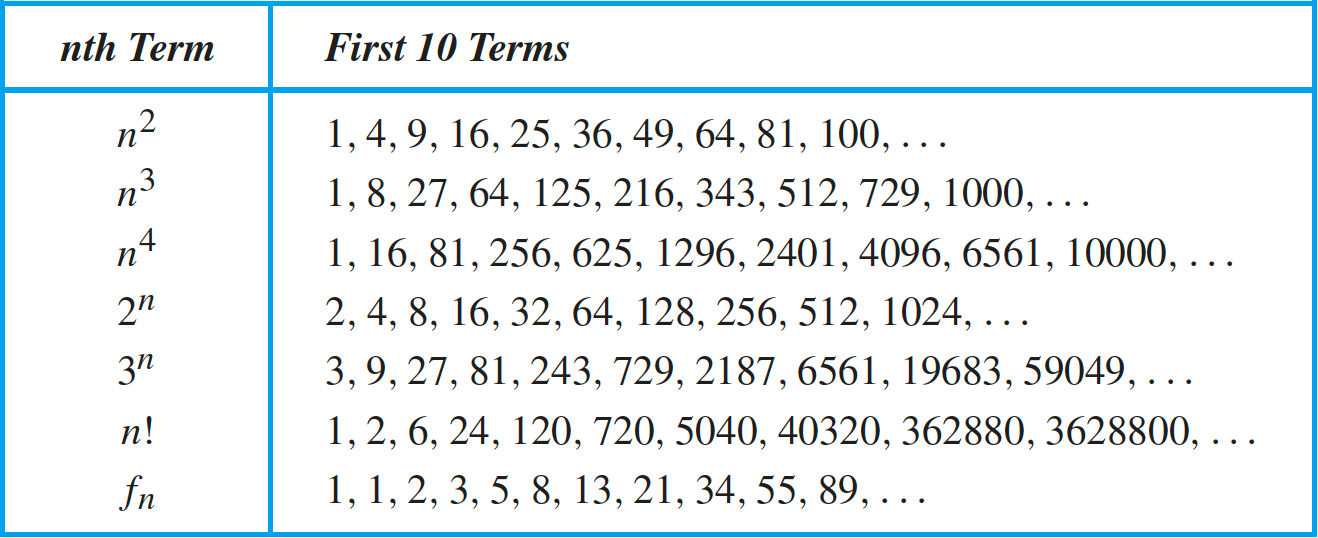
\includegraphics [width=5in]{Table-2-4-1-SomeUsefulSequences}
   \caption{Some Useful Sequences}
   \label{table:Some Useful Sequences}
   \end{table}

The reader interested in integer sequences will want to look at the Online Encyclopedia of Integer Sequences originally created by Neil Sloane and available online.

\subsection{Strings}
Sequences sometimes have a co-domain of symbols that can be listed in a sequence such that each symbol is a distinct symbol. This allows sequences of symbols to be represented without commas without confusion. The set of symbols is usually called the alphabet and commonly represented with the capital sigma, $\Sigma$. Finite equences of symbols are called strings and represented by $a_1a_2a_3 \ldots a_n$ 


\subsection{Evaluation of Functions}
Note that functions have one notation that just gives the function a name and identifies the domain and codomain but does not define how one maps to the image given the pre-image. 
Some functions are trivially evaluated. The other notation defines how that is done and it is often a mathematical expression. But it need not be. It can be any procedure that will ensure a value from the codomain is returned when requested. 

This has a historical point. Prior to the middle of the 20c the word computer was a job description not a machine. It was the job of the mathematician to give the computers the instructions on how to compute the functions that were needed. More often than not these values were compiled into books and used as reference when the function needed to be evaluated. Turing was one of the first to ask what limits a machine would have if the mathematician gave instructions that could be executed by a machine. We now call these procedures the algorithms that are used to evaluate a function given it aguments. 




\section {Sigma Notation, Summations and Open Form Formulas}
Given a function which produces a sequence, one operation we frequently wish to do is sum the terms. We define notation for this.

\begin{definition} [Summation] \index{summation}
Given a sequence $\{a_n\}$, we use the notation $\sum_{j=m}^{n} a_j $ to represent $a_m + a_{m+1}+ ... + a_n$. The variable $j$ is called the \textit{index of summation}, the value $m$ the  \textit{lower limit} and the value $n$ the \textit{upper limit}. 
\end{definition}

Shift the index of summation. 
Ex: What is the evaluation of $\sum_{j=1}^5 j^2$ with an index of summation that runs from 0 to 4 instead of 1 to 5? Substitute $k=j-1$ so the old index of summation would run from 1 to 5 but the new index of summation will run from  0 to 4 and the new summand will be $(k+1)^2$.
Sol: 

\subsection{Properties of Summation}

\begin{align}
\sum_{i=m}^n ca &=  c \sum_{i=m}^n a\\
\sum_{i=m}^n (a \pm b) &= \sum_{i=m}^n a \pm  \sum_{i=m}^n b \\
\sum_{i=m}^n a &= \sum_{i=m+p}^{n+p} a
\end{align}



It may start at something other than 1 and may sum to infinity. The letter $j$ is called the \textit{index of summation}, and the choise of the letter $j$ as variable is arbitrary; that is, we could have used any other letter, such as $i$ or $k$. Or, in notation, 
$$\sum_{j=m}^n a_j = \sum_{i=m}^n a_i = \sum _{k=m}^n a_k$$
where $m$ is the \textbf{lower limit} and $n$ is the \textit{upper limit}.

\subsection{Closed form solution}
For finite sequences, it is always possible to add the terms to calculate the sum. But these sequences can be very long making the summation an expensive operaton. And it is impossible if the sequence is infinite. Another way must be found and this brings us to closed form solutions. Many summations can be restated as formulas that are functions of the upper limit of summation. These are less burdensome computationally and are possible for infinite sequences with calculus.  
A closed form soluiton will have a finite number of operations and does not require the articulation of every term of the sequence.

\begin{theorem}
If $a$ and $r$ are real numbers with $r\ne 0$, then
\[   
\sum_{j=0}^n ar^j  = 
     \begin{cases}
       \frac{ar^{n+1}-a}{r-1}, &\quad\text{if $r \ne 1$,}\\ 
       $(n+1)a$,               &\quad\text{if $r=1$.} \\
     \end{cases}
\]
\end{theorem}

telescoping

\subsection{Useful Closed Form Solutions}
\begin{align}
\sum_{k=1}^n k & = \frac{n(n+1)}{2}\\
\sum_{k=1}^n k^2 & =\frac{n(n+1)(2n+1)}{6}\\
\sum_{k-1}^n k^3 & =\frac{n^2(n+1)^2}{4}\\
\sum_{i=0}^n 2^i & = 2^0+2^1+\dots 2^{n-1}+2^n= 2^{n-1} -1
\end{align}


\section {Growth of Functions and Asymptotic Notation}
As we saw when we talked about the graphs of common graphs  (Figure \ref{figure:GraphsOfCommonFunctions}) we see that there is a difference among these functions in how quickly the function values climb as the argument, $n$, grows. For example you know that a quadratic polynomial will overtake a linear polynomial. But many linear functions will evaluate to higher numbers for small values. We want some way to express the concept that a quadratic is in some sense bigger. This leads to a new notation, the Big-O or asymptotic notation or \textbf{Bachmann-Landau notation} and the $O$ is sometimes called the \textbf{Landau} symbol. Knuth extended this notation in his work.
Characterize functions according to their growth rates. different functions with the same growtwth rate may be represented using the same O notaiotn. the order of the function. O is used to specify an upper growth bound. Since a slower growing function may give a higher value for low values of the argument but pull ahead and forever remain ahead for large values, it is not sufficient to offer a few values to demonstrate. 

\begin{definition}
Let $f$ and $g$ be functions fromthe set of integers or reals to the set of real numbers. We say that $f(n)$ is $O(g(n))$ if there are constants $C$ and $k$ such that 
\begin{displaymath}
\lvert f(x)\rvert \le C\lvert g(n)\rvert
\end{displaymath}
whenever $n>k$. We read this as ``$f(n)$ is big-oh of $g(n)$''. The constants $C$ and $k$ are called the \textbf{witnesses} to the relationship $f(n)$ is to $O(g(n))$. To demonstrate that $f(n)$ is big-oh  we only need to produce one set of witnesses. Note that it is an abuse of the notation to say $f(n)=O(g(n))$ since no equality is established, only an assertion that the functions belong to the same class of functions. 
\end{definition}

$$f(n) = O(g(n)) \text{ as } n\rightarrow \infty$$
if and only if for all sufficiently large values of $n$, the absolute value of $f(n)$ is at most a positive constant multiple of another function $g(n)$. That is $f(n)=)(g(n))$ if and only if there existss a positive realy number C and a real number $n_0$ such that
$$\lvert f(n) \rvert \le cg(n) \text{for all } n\ge n_0$$
Instead of looking at at the function itself, it is helpful to look at a function as a family of functions. For a linear function $f(n)=n$ we can define a set of functions based on that by introducing constants $c_0$ and $c_1$ like this: $f(n)=c_1n+c_0$. This can be done for all the common functions giving us this list:\\
$
\begin{array}{lll}
\text{log} &  O (\log n) & \\
\text{log linear} & O(n \log n) & \\
\text{linear} & O(n)& c_1n+c_0\\
\text{quadratic} &On^2& c_2n^2 +c_1n + c_0 \\
\text{cubic}&O(n^3) & c_3n^3 + c_2n^2 + c_1n + c_0\\
\text{exponential} &O(2^n) & \\
\text{factorial} & O(n!) &
\end{array}
$

If there are constants such that a function can be restated as one of these families of functions then we say it is \textit{of the same order of magnitude} as 

Given two linear polynomial equations, we can always do this by changing the values of the constants. But no matter how you change the constants of a linear polynomial, a quadratic polynomial will always overtake it. This shows that a quadratic will ALWAYS beat a linear function, that they are in some sense in different categories regardless of the choice of constants. This gives us the concept of the category of the function or the order or magnitude designated by Big O. We can change any linear function into another linear polynomial function by changing the constants. We group all of these together and call them linear polynomial functions or polynomial functions on n, written O(n). We can prove that there are at least 7 categories that are important to the study of computer science, constant O(1), linear O(n), log O(log n), log-linear O(n log n), quadratic O(n**2), exponential O(2**n), and factorial O(n!). Note that each of these is a grouping of functions that include all the variations of different constants. By choosing the constants, we can always find some n sub 0 such that a quadratic will beat a linear. This gives us an ordering of these categories

$O(1) < O(\log n) < O(n) < O(n \log n) < O(n^2) < O(2^n) < O(n!)$

For any two specific functions of different categories one can find the n sub 0 at which the larger function overtakes the smaller and forever remains ahead. This way of viewing the relative size of functions will be used when we study the complexity of algorithms later.

\begin{theorem}
Let 
\begin{displaymath}
p(n)=a_kn^k+a_{k-1}n^{k-1}+\ldots +a_1n^1+a_0
\end{displaymath}
be a polynomial in $n$ of degree $k$, where each $a_i$ is nonnegative. Then
\begin{displaymath}
p(n)=\Theta(n^k).
\end{displaymath}
\begin{proof}

\end{proof}
\end{theorem} 


\begin{definition}[Big-Omega]
Let $f$ and $g$ be functions from the set of integers or reals to the set of reals. We say that $f(n)$ is $\Omega(g(n))$ if there are positive constants $C$ and $k$ such that 
\begin{displaymath}
\lvert f(n)\rvert \ge C\lvert g(n)\rvert
\end{displaymath}
whenever $x>k$. Read this as ``$f(n)$ is big-Omega of $g(n)$''.
\end{definition}

\begin{definition}[Big Theta]

\end{definition}

\newpage
